\tp[Propri�t�s des intensit�s et des tensions]{Propri�t�s des intensit�s \\et des tensions}

\nomprenomclasse

\objectifs{
\item R�aliser un sch�ma de montage o� figurent les appareils de mesure (amp�rem�tre, voltm�tre) et leurs bornes
\item \'Etude des propri�t�s de l'intensit� d'un courant dans un circuit �lectrique
\item \'Etude des propri�t�s de la tension dans un circuit �lectrique
}


\materiel{
\item g�n�rateur $6$-$12~V$ r�glable
\item 3 multim�tres
\item 2 lampes de tension nominale $6~V$
\item $R = 10~\Omega$ ; $R_1 = 180~\Omega$ ; $R_2 = 270~\Omega$
\item 1 bouton poussoir
}

\section{\'Etude de l'intensit�}

\subsection{Circuit s�rie}

%\begin{center}
%\includegraphics[width=7cm]{montage_serie_i.eps}
%\end{center}

\begin{center}
\begin{pspicture}(0,0)(6,3)
%\psgrid[subgriddiv=1,griddots=10]
\pnode(0,2.5){B}
\pnode(6,2.5){A}
\battery(B)(A){$E$, $r$}
\pnode(0,0.5){C}
\pnode(6,0.5){D}
%\wire(A)(D)
\switch[intensitylabel=$I_3$](D)(A){$K$}
\wire(C)(B)
\pnode(3,0.5){CD1}
\resistor[intensitylabel=$I_1$](C)(CD1){$R$}
\lamp[intensitylabel=$I_2$](CD1)(D){$\mathcal L$}
\end{pspicture}
\end{center}

\begin{enumerate}
\item Faire un sch�ma de montage pour chaque cas permettant la :


\begin{enumerate}
\item Mesure de $I_1$
\item Mesure de $I_2$
\item Mesure de $I_3$
\end{enumerate}

\item Faire le montage permettant la mesure de $I_1$. Faire v�rifier le montage. Mesurer $I_1$.
\item Faire le montage permettant la mesure de $I_2$. Faire v�rifier le montage. Mesurer $I_2$.
\item Faire le montage permettant la mesure de $I_3$. Faire v�rifier le montage. Mesurer $I_3$.
\item Conclure.
\end{enumerate}

\pagebreak[3]

\subsection{Circuit d�rivation}

%\begin{center}
%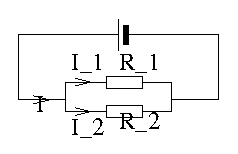
\includegraphics[width=7cm]{montage_deriv_i.eps}
%\end{center}

\begin{center}
\begin{pspicture}(0,-1)(6,3)
%\psgrid[subgriddiv=1,griddots=10]
\pnode(0,3){B}
\pnode(6,3){A}
\battery(B)(A){$E$, $r$}
\pnode(0,0.5){C}
\pnode(6,0.5){D}
\wire(C)(B)
\switch(D)(A){$K$}
\pnode(1.5,0.5){CD1}
\pnode(4.5,0.5){CD2}
\resistor[parallel,parallelarm=1,parallelsep=2,intensitylabel=$I_1$,dipoleconvention=receptor](CD2)(CD1){$R_1$}
\resistor[parallel,parallelarm=-1,parallelsep=2,intensitylabel=$I_2$,dipoleconvention=receptor](CD2)(CD1){$R_2$}
\wire[intensitylabel=$I$](C)(CD1)
\wire(CD2)(D)
\end{pspicture}
\end{center}


\begin{enumerate}
\item Faire un sch�ma de montage permettant de mesurer $I$, $I_1$ et $I_2$.
\item R�aliser le montage. Faire v�rifier le montage.
\item Mesurer $I$, $I_1$ et $I_2$.
\item Conclure.
\end{enumerate}



\section{\'Etude de la tension}
\subsection{Circuit s�rie}

\begin{center}
\begin{pspicture}(0,0)(12,5)
%\psgrid[subgriddiv=1,griddots=10]
\pnode(0,4.5){B}
\pnode(12,4.5){A}
\battery[tensionlabel=$U$](B)(A){$E$, $r$}
\pnode(0,0.5){C}
\pnode(12,0.5){D}
%\wire(A)(D)
\switch(D)(A){$K$}
\wire(C)(B)
%\pnode(4,0.5){CD1}
%\pnode(8,0.5){CD2}
%\resistor[tensionlabel=$U_1$](C)(CD1){$R_1$}
%\resistor[tensionlabel=$U_2$](CD1)(CD2){$R_2$}
%\resistor[tensionlabel=$U_3$](CD2)(D){$R_3$}
\pnode(6,0.5){CD1}
\resistor[tensionlabel=$U_1$](C)(CD1){$R_1$}
\resistor[tensionlabel=$U_2$](CD1)(D){$R_2$}
\end{pspicture}
\end{center}


\begin{enumerate}
\item Faire un sch�ma de montage permettant de mesurer $U$, $U_1$ et $U_2$.
\item R�aliser le montage. Faire v�rifier le montage.
\item Mesurer $U$, $U_1$ et $U_2$.
\item Conclure.
\end{enumerate}

\subsection{Circuit d�rivation}

\begin{center}
\begin{pspicture}(0,-0.5)(6,8)
%\psgrid[subgriddiv=1,griddots=10]
\pnode(0,8){B}
\pnode(6,8){A}
\battery[tensionlabel=$U$](B)(A){$E$, $r$}
\pnode(0,0){C}
\pnode(6,0){D}
\wire(C)(B)
\switch(6,4)(A){$K$}
%\resistor[tensionlabel=$U_1$,dipoleconvention=receptor](0,0)(6,0){$R_1$}
%\resistor[tensionlabel=$U_2$,dipoleconvention=receptor](0,2)(6,2){$R_2$}
%\resistor[tensionlabel=$U_3$,dipoleconvention=receptor](0,4)(6,4){$R_3$}
\resistor[tensionlabel=$U_1$,dipoleconvention=receptor](0,0)(6,0){$R_1$}
\resistor[tensionlabel=$U_2$,dipoleconvention=receptor](0,2)(6,2){$R_2$}
\wire(6,4)(D)
\end{pspicture}
\end{center}

\begin{enumerate}
\item Faire un sch�ma de montage permettant de mesurer $U$, $U_1$ et $U_2$.
\item R�aliser le montage. Faire v�rifier le montage.
\item Mesurer $U$, $U_1$ et $U_2$.
\item Conclure.
\end{enumerate}